
\section{Effect of MEC on the reconstructed energy distribution}
\label{app:effect_mec_ereco}

The second reason is given by the MEC systematic parameter.
As written above, the uncertainty on MEC is as large as 102\%.
If the pre-BANFF systematics are used the nominal value is 0.27
and large fraction of the possible random extraction within $1\sigma$ 
is not allowed because in the unphysical region. 
Indeed the MEC parameter is a normalization parameter which cannot
have negative values. 
If post-BANFF systematics are used the uncertainty remains still close to 100\%,
because the oxygen parameters are not constrained by the BANFF fit, 
but the nominal value changes to 1.031,
as shown in table~\ref{tab:banff_uncertainties}.
Since all the random extractions within $1\sigma$ is still in the physical region,
the MEC distribution becomes less asymmetric as well as the effect on the 
reconstructed energy distribution.
It becomes more clear when looking to figures~\ref{fig:mec_extraction},
~\ref{fig:mec_total_events} and~\ref{fig:mec_error_envelope}.

\begin{figure}
\center
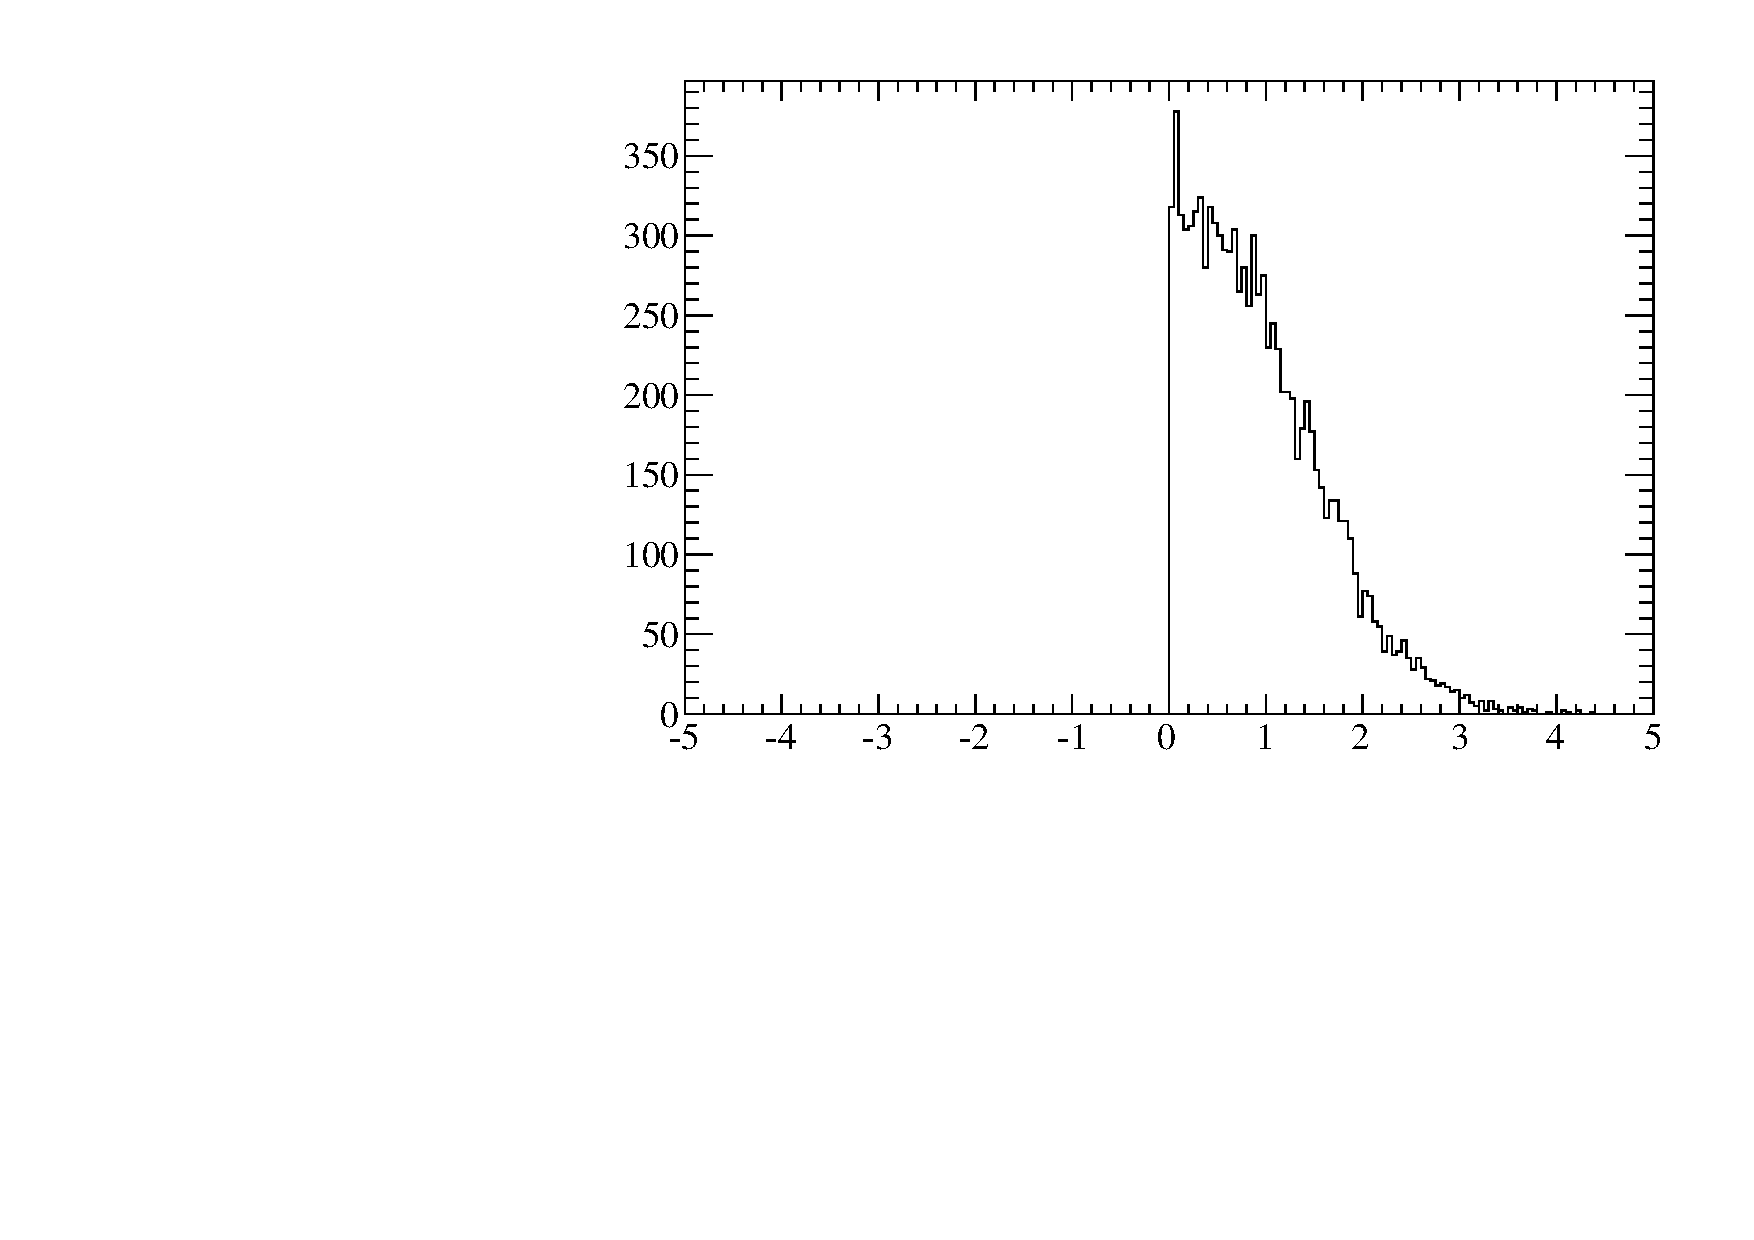
\includegraphics[width=0.48\linewidth]{./nuebar_plots/spectrum_tweaked/MEC/extraction_MEC_prefit.pdf}
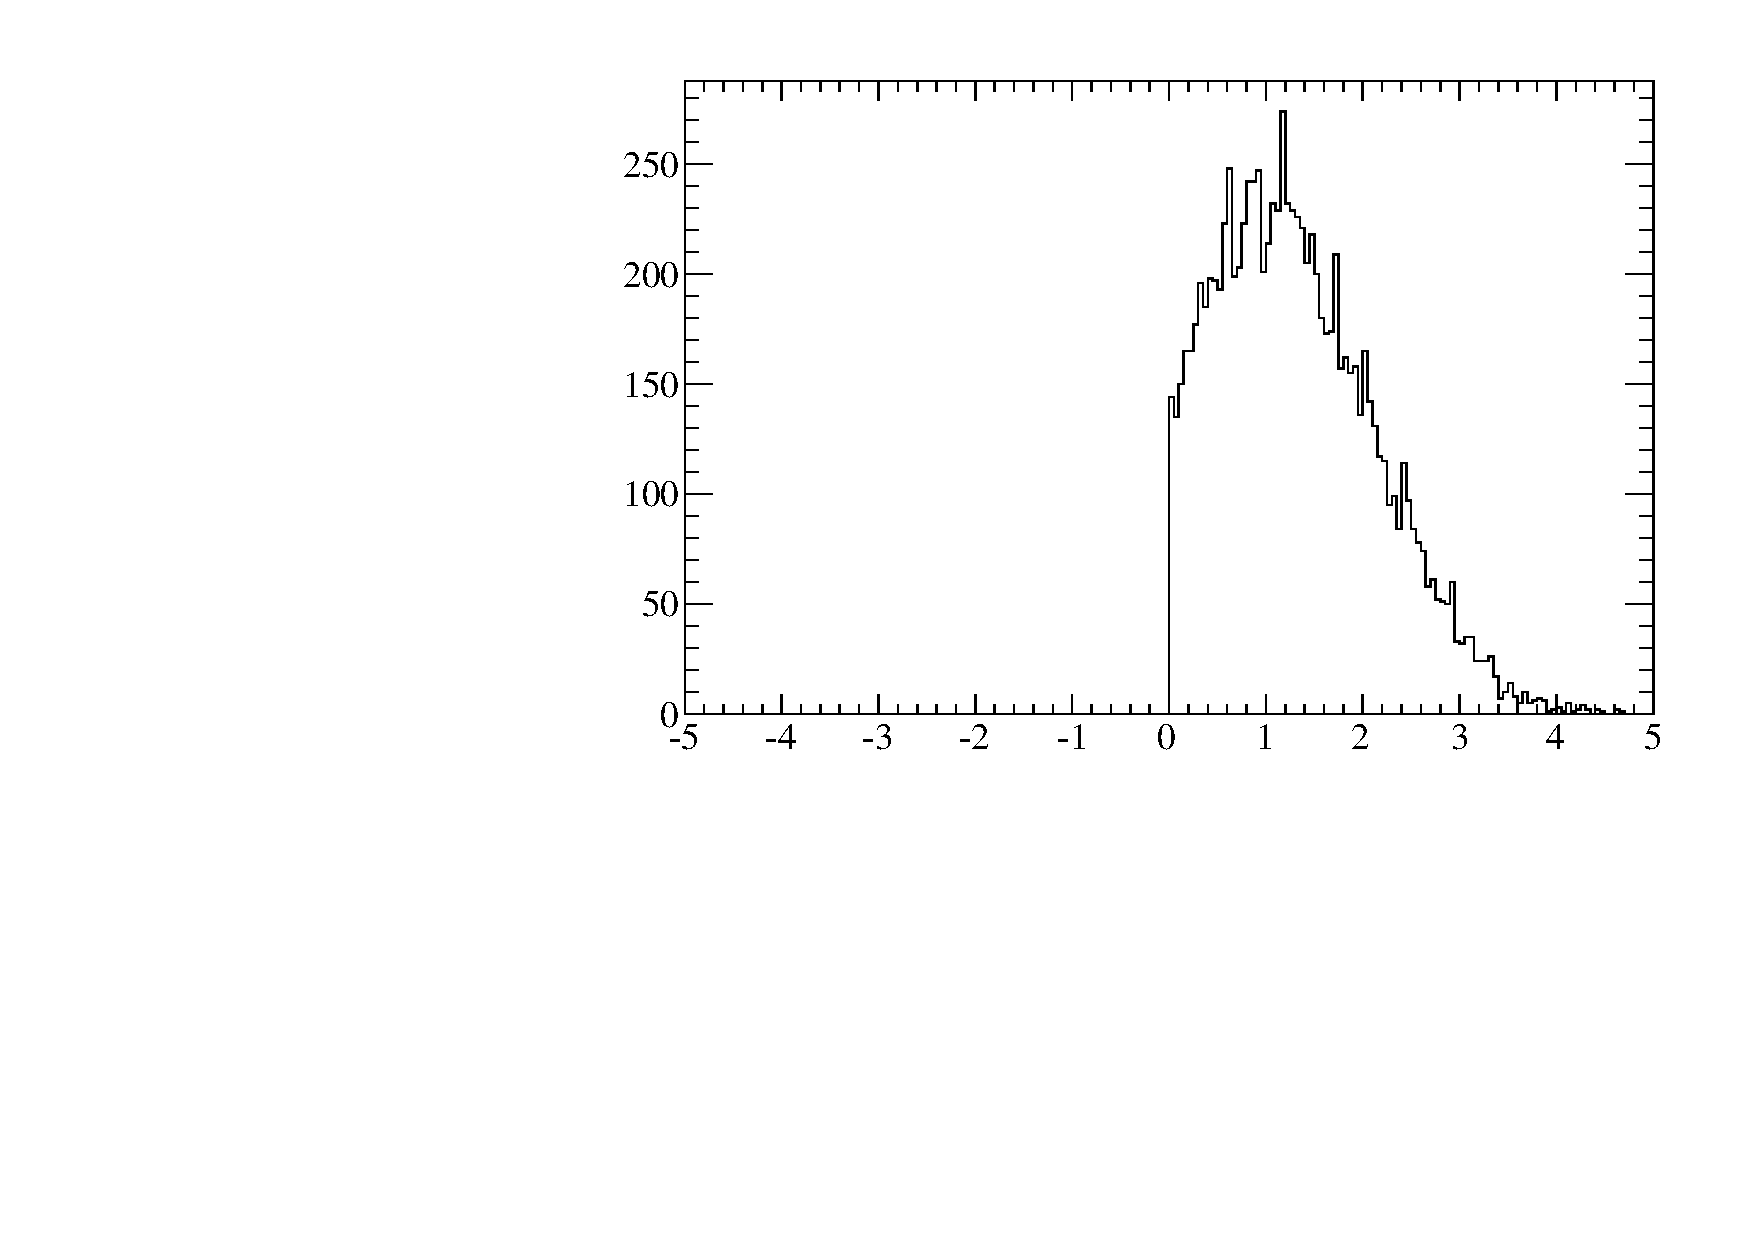
\includegraphics[width=0.48\linewidth]{./nuebar_plots/spectrum_tweaked/MEC/extraction_MEC_postfit.pdf}
\caption {
Distribution of the MEC oxygen parameter obtained by \NumToys toys for 
pre-BANFF (left) and post-BANF (right) systematics.
All the other systematic parameters are fixed to the nominal values.
}
\label{fig:mec_extraction}
\end{figure}

\begin{figure}
\center
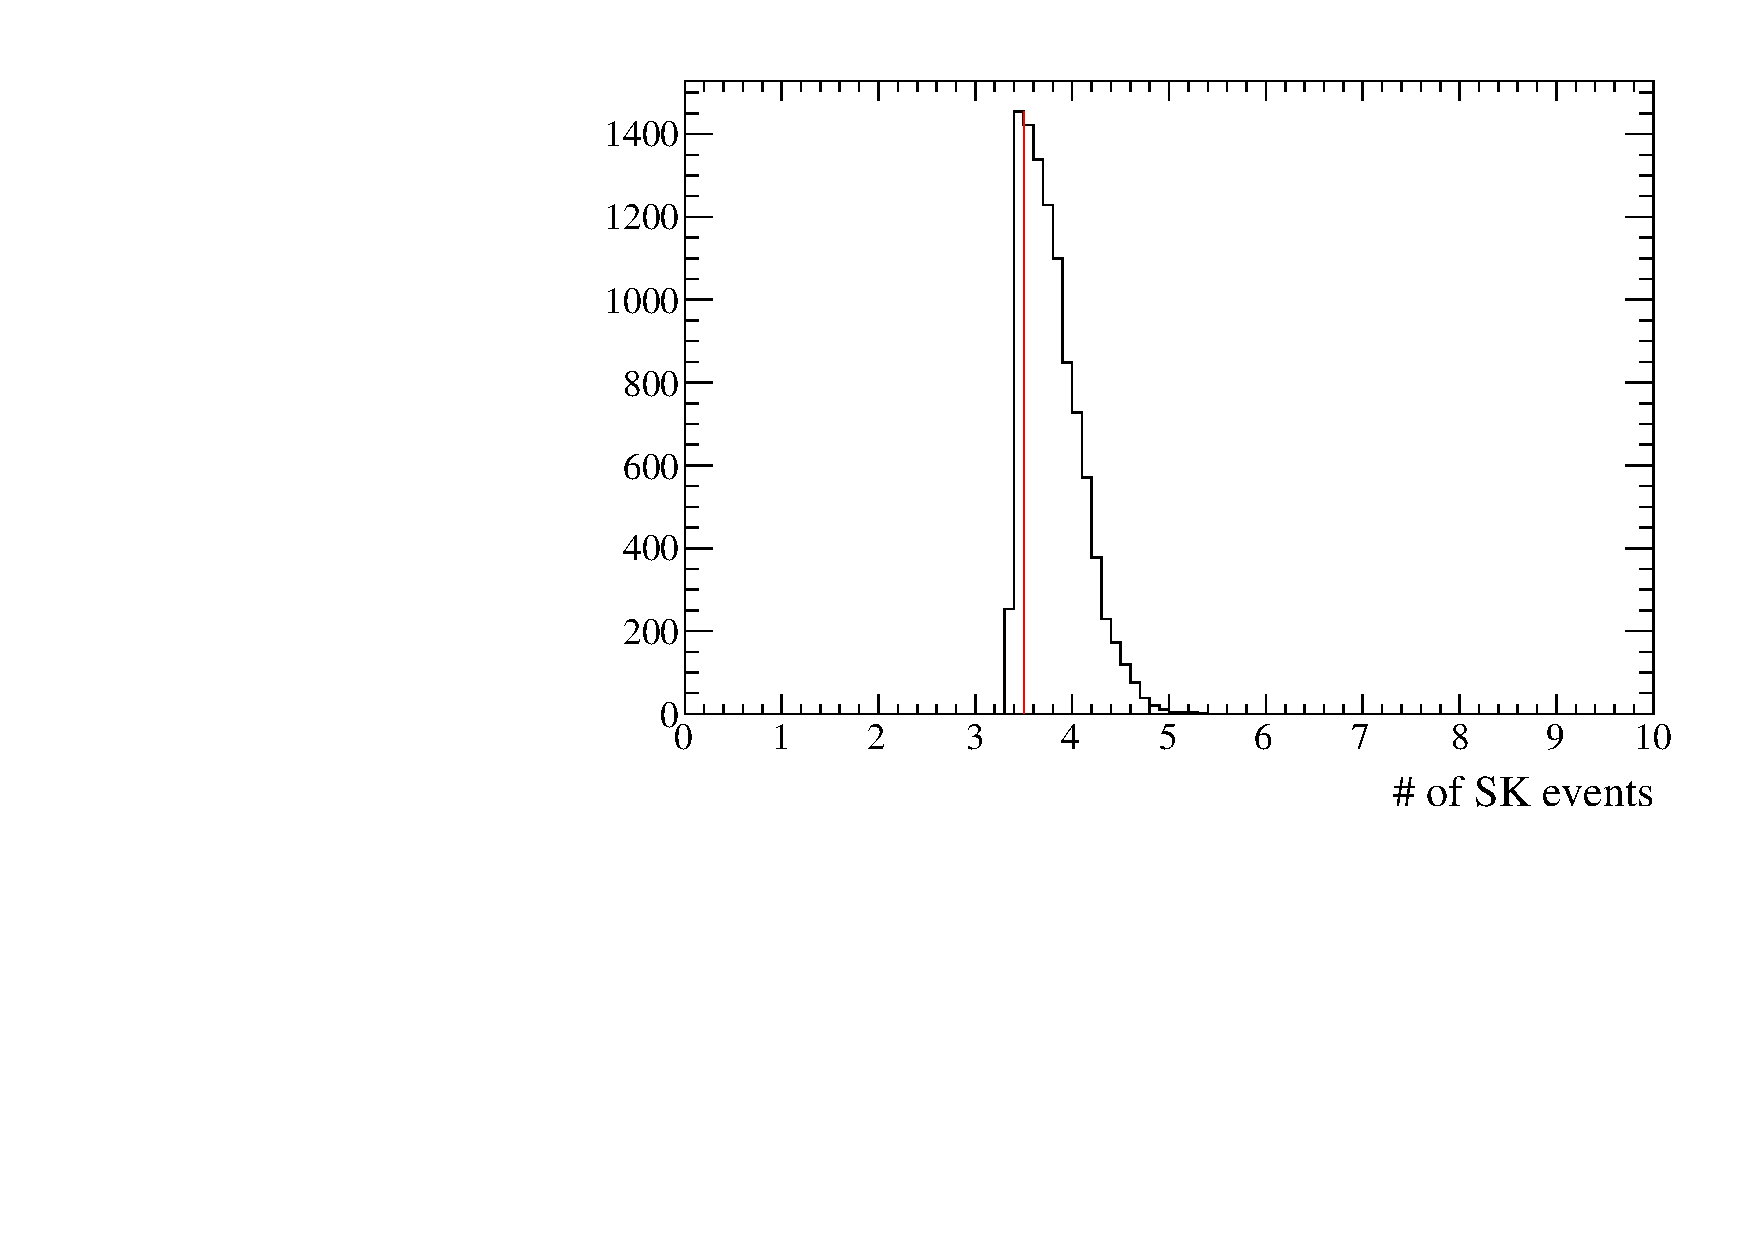
\includegraphics[width=0.48\linewidth]{./nuebar_plots/spectrum_tweaked/MEC/total_event_MEC_prefit.pdf}
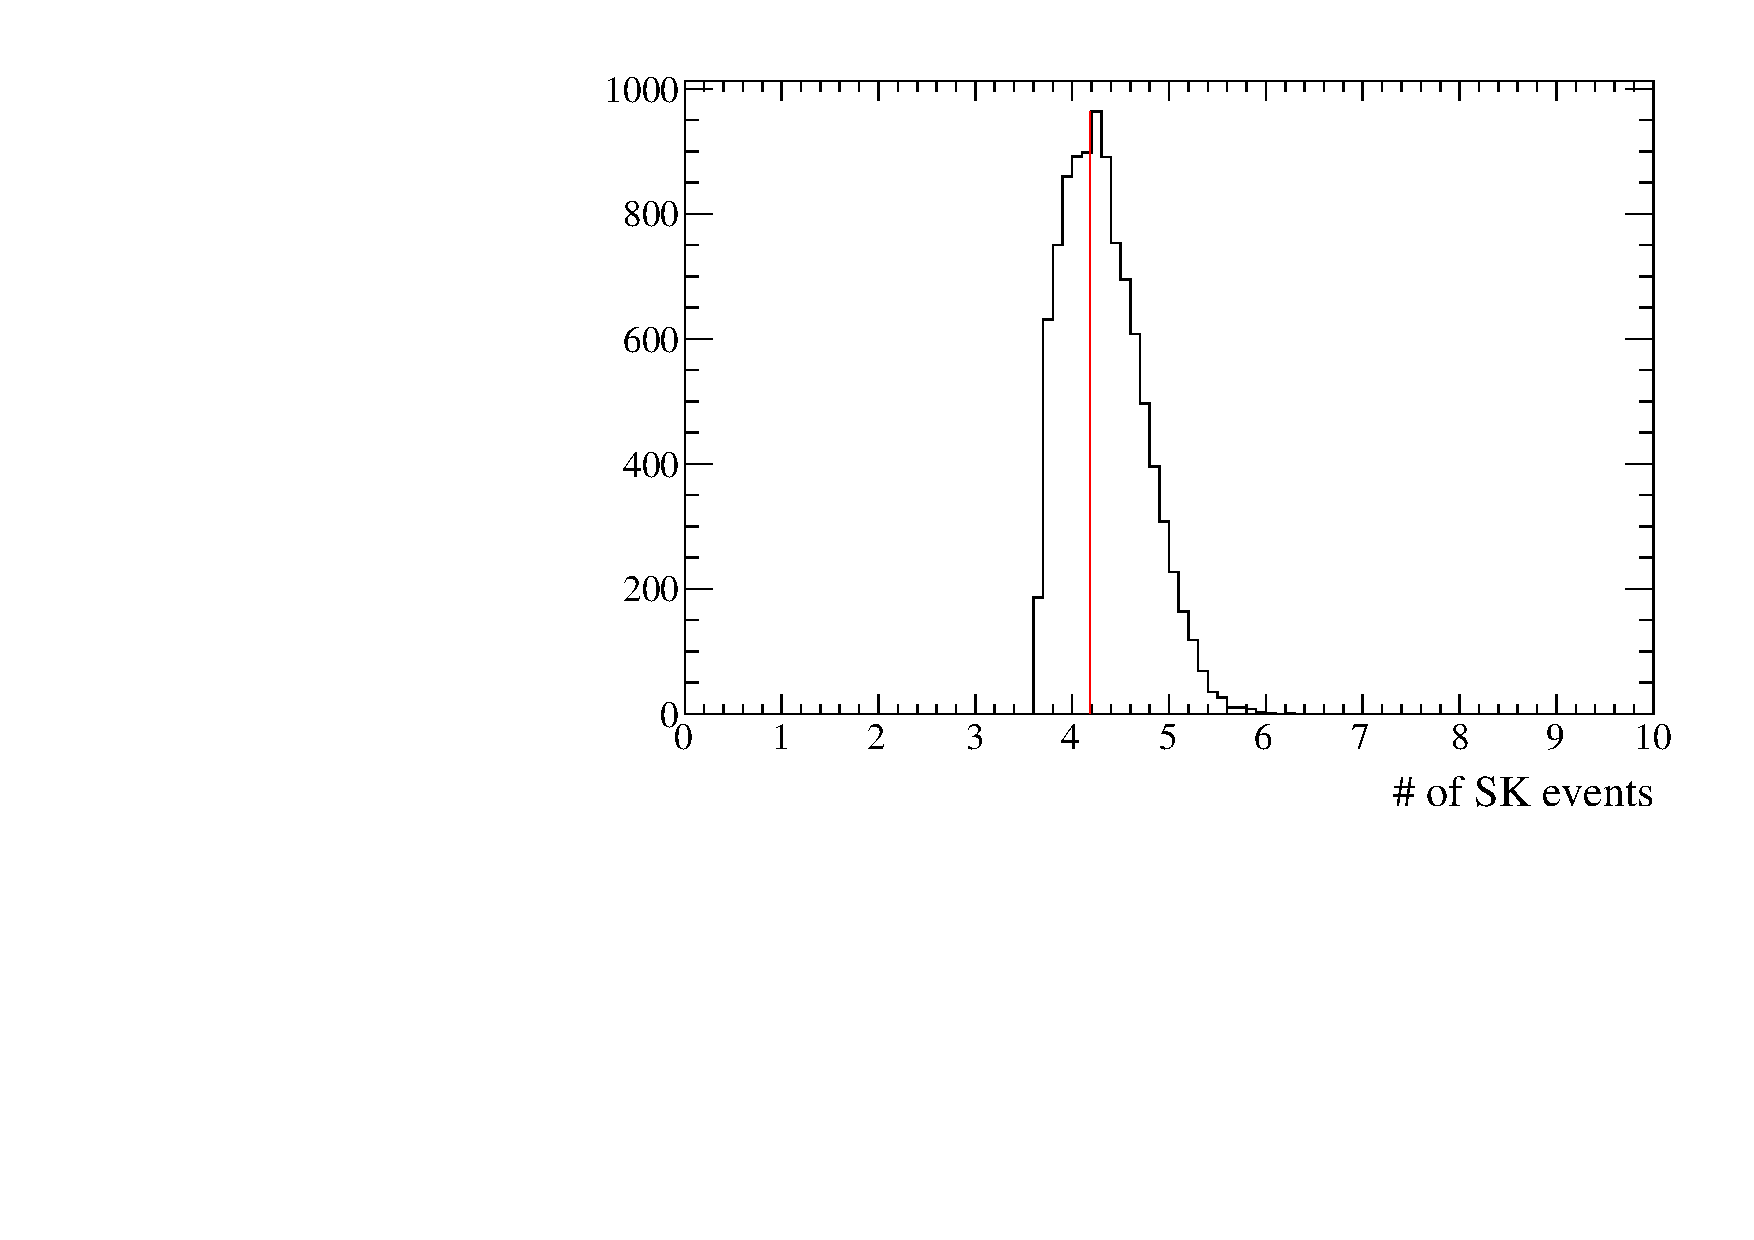
\includegraphics[width=0.48\linewidth]{./nuebar_plots/spectrum_tweaked/MEC/total_event_MEC_postfit.pdf}
\caption {
Distribution of the total superK number of events obtained by making \NumToys toys
where only the MEC oxygen parameter is randomly extracted and 
all the other systematic parameters are fixed to the nominal values. 
The red line correspond to the Asimov dataset where the MEC parameter is fixed
to its nominal value.
Pre-BANFF is shown on the left, 
while post-BANF is shown on the right.
}
\label{fig:mec_total_events}
\end{figure}


\begin{figure}
\center
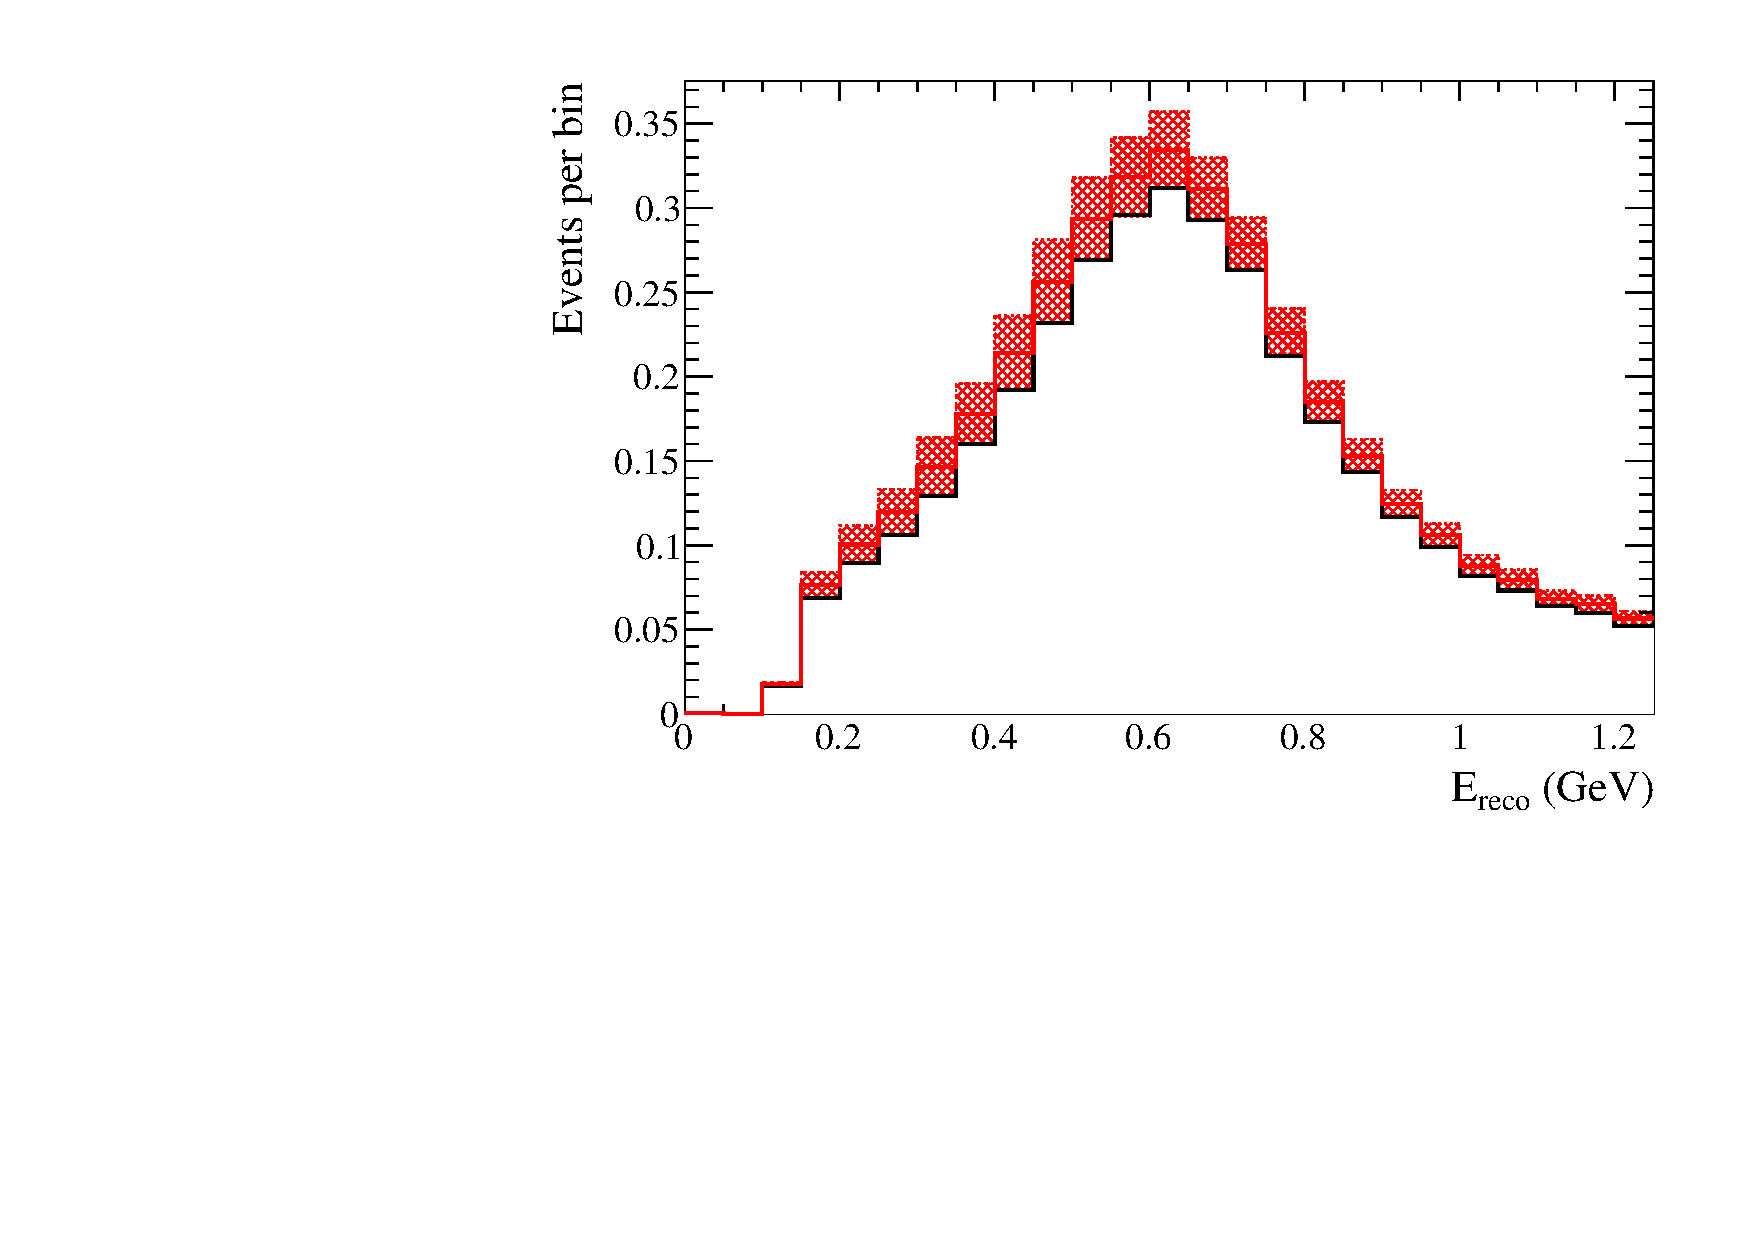
\includegraphics[width=0.48\linewidth]{./nuebar_plots/spectrum_tweaked/MEC/error_envelope_MEC_prefit.pdf}
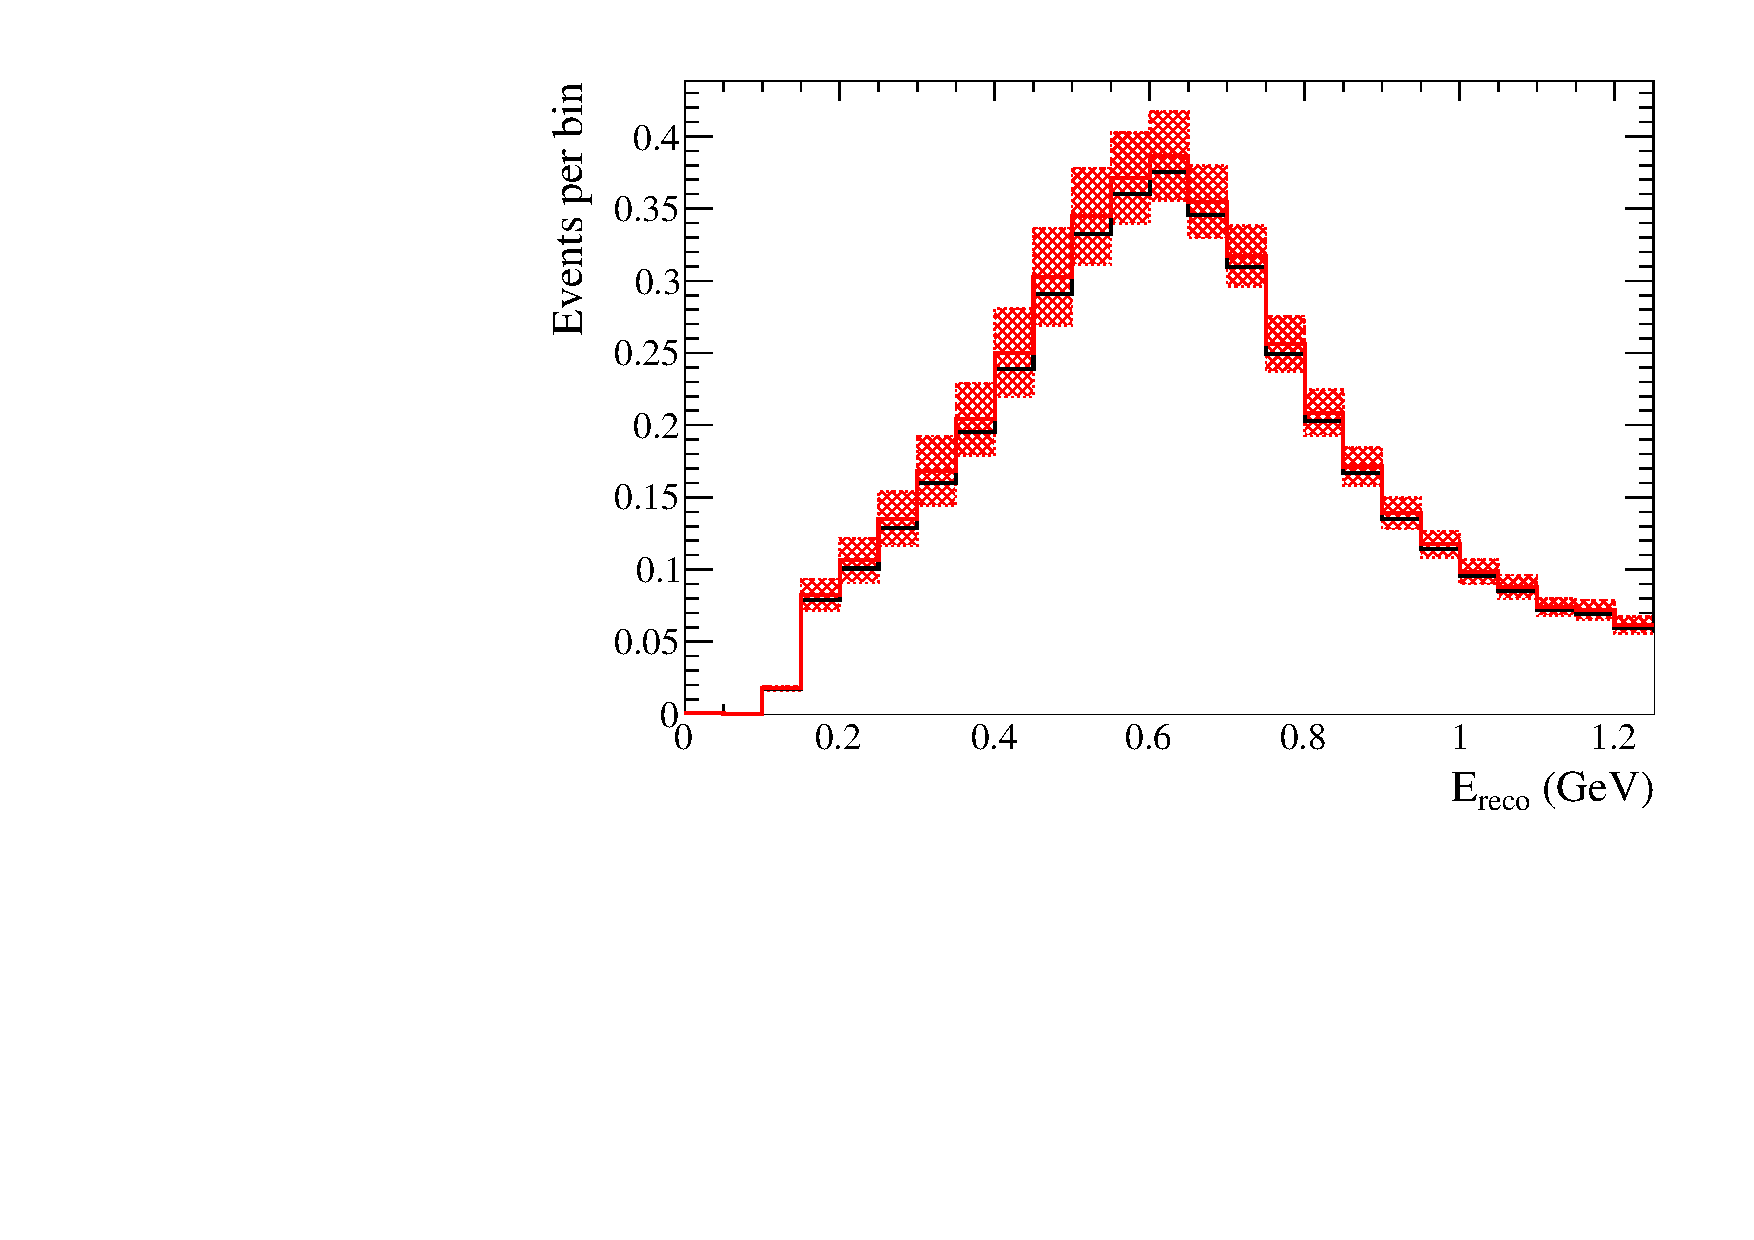
\includegraphics[width=0.48\linewidth]{./nuebar_plots/spectrum_tweaked/MEC/error_envelope_MEC_postfit.pdf}
\caption {
Reconstructed energy distribution obtained by making \NumToys toys
where only the MEC oxygen parameter is randomly extracted and 
all the other systematic parameters are fixed to the nominal values. 
The red line correspond to the Asimov dataset where the MEC parameter is fixed
to its nominal value.
The error envelopes in each bin correspond to the $1\sigma$ error 
obtained from the distribution of the extracted number of events.
First the median (red line) is found. 
Then the upper (lower) error corresponds
to the number of events for which the 34\% of toys is contained between it and the median
on the right (left) side.
The black line shows the expected nominal reconstructed energy distribution.
Pre-BANFF is shown on the left, 
while post-BANF is shown on the right.
}
\label{fig:mec_error_envelope}
\end{figure}

















\clearpage


